
%%%%%%%%%%%%%%%%%%%%%%%%%%%%%%%%%%%%%%%%%%%%%%%%%%%%%%%%%%%%%%%%%%%%%%%%%%%%%%%%%%%%%%%%%%%%%%%%%%%%%%%%%%%%%%%%%%%%%%%%%%%%%%%%%%%%%%%%%%%%%%%%%%%%%%%%%%%%%%%%%%%%
\chapter{How do I analyse micro-array data using Ondex?}
\label{cha:pie}
%%%%%%%%%%%%%%%%%%%%%%%%%%%%%%%%%%%%%%%%%%%%%%%%%%%%%%%%%%%%%%%%%%%%%%%%%%%%%%%%%%


\section*{Application case: Analysing Experimental Data in the context of Integrated Biological Networks}
\label{sec:pie_charts_app}

We integrated AraCyc (\url{http://www.arabidopsis.org/biocyc/index.jsp}), a database containing pathway information for the plant 
\textit{Arabidopsis thaliana}, with data from the former DRASTIC-INSIGHT database for information on plant gene expression. 
Additionally, we loaded micro-array expression data onto the concepts of the network using attributes. 
(A workflow named pathways\_expdata\_integrator\_workflow.xml is available under Tutorial\_files/Application\_cases for this data integration pipeline).
The expression data has been analysed for statistical significance and normalized.
We show that an integrative approach to the exploration of micro-array expression data can leverage the understanding in the context of pathways 
and might yield new biological insights.
\begin{figure}[H]
\centering
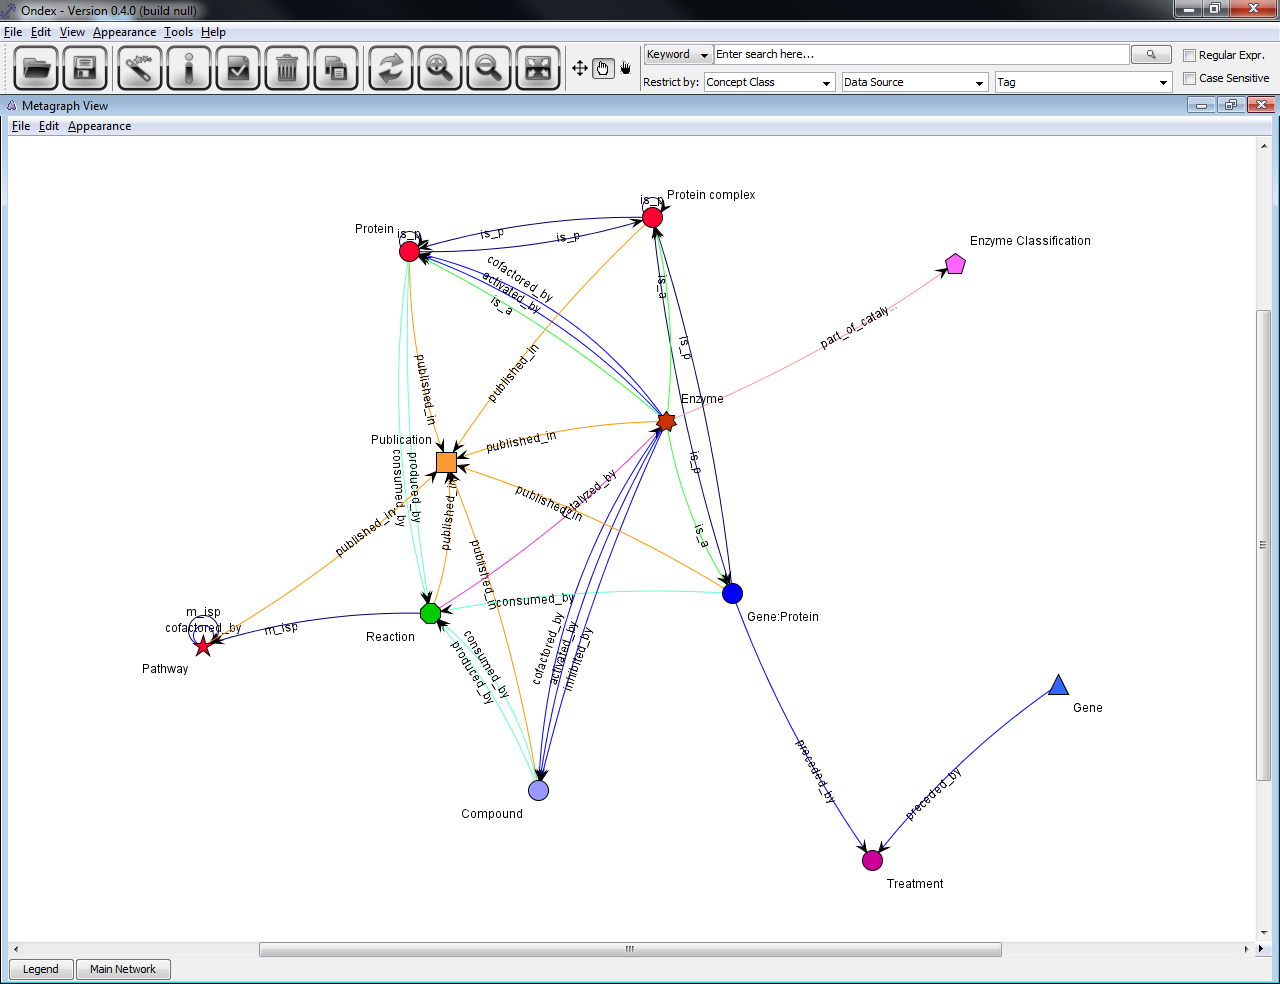
\includegraphics[scale=0.35]{images/Oct12/app1fig1.png} 
\caption{Metagraph}
\label{fig:metagraph_pathways}
\end{figure}
After loading the data file Tutorial\_files/Application\_cases/pathways\_expdata.oxl, a metagraph is displayed in Figure \ref{fig:metagraph_pathways}.
The different concept classes are:
\begin{itemize}
\item Genes from the DRASTIC database, which did not map to any AraCyc genes
\item Treatments (e.g. drought, ABA) from the DRASTIC database under which a gene showed a significant change in expression
\item Merged entities consisting of Genes from DRASTIC and Proteins from AraCyc together with microarray expression data to achieve a more compact pathway representation
\item Protein complexes described in AraCyc
\item Proteins in AraCyc, for which there is no expression data available
\item Enzymes catalysing reactions from AraCyc
\item Enzyme classifications for enzymes from AraCyc
\item Chemical compounds involved with reactions and enzymes in AraCyc
\item Reactions belonging to an AraCyc pathway
\item AraCyc pathways which can be part of a hierarchy
\item Publications assigned to entries in AraCyc
\end{itemize}

\begin{figure}[H]
\centering
\subfigure[Metadata - Concept Classes tab]{
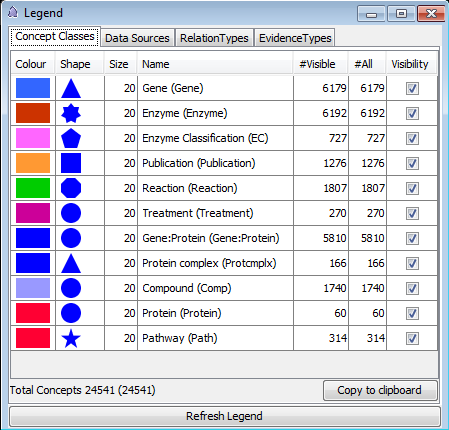
\includegraphics[scale=0.5]{images/Oct12/app1fig2_1.png} 
\label{fig:CCs}
}
\subfigure[Metadata - Relation Types tab]{
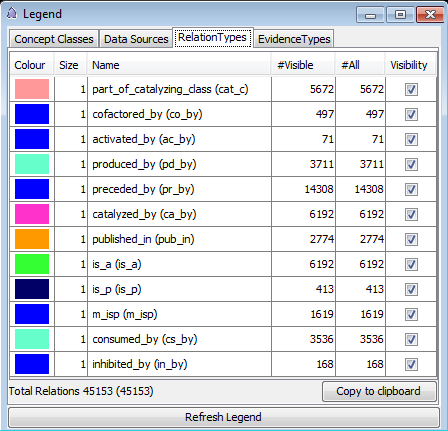
\includegraphics[scale=0.5]{images/Oct12/app1fig2_2.png} 
\label{fig:RTs}
}
\label{fig:metadata_pathways}
\caption{Metadata - legend and numbers}
\end{figure}
The whole network contains 24541 concepts and 45153 relations as shown in Figure \ref{fig:metadata_pathways}. 
Using tag information we can display only the relevant sub-network instead of having to work with the whole network.

\begin{figure}[H]
\centering
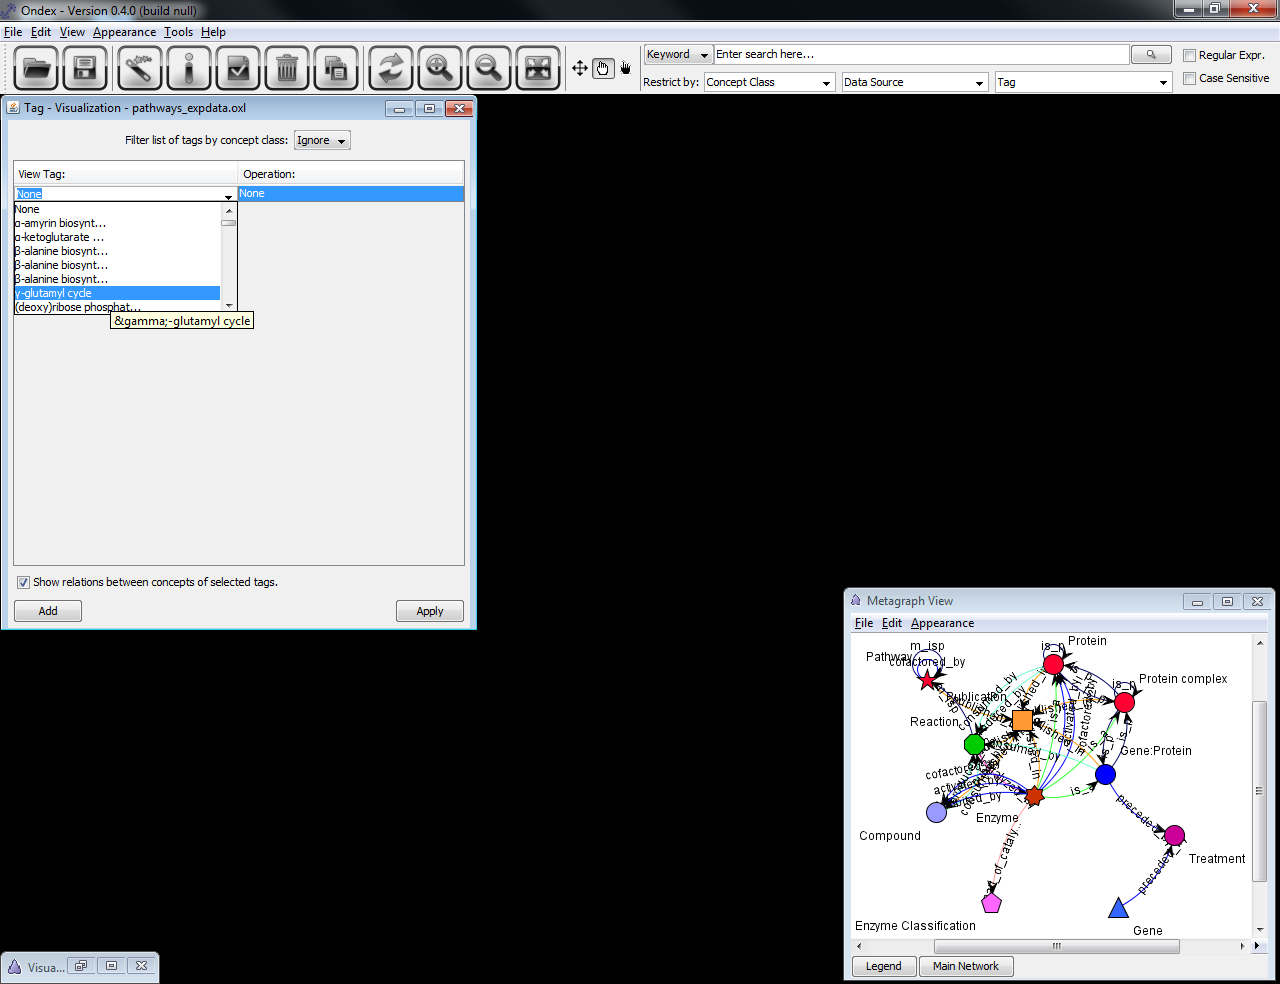
\includegraphics[scale=0.35]{images/Oct12/app1fig3.png} 
\caption{Tag filter}
\label{fig:tag_filter}
\end{figure}

From the tag drop-down list please select gamma-glutamyl-cycle as shown in Figure \ref{fig:tag_filter}.
The resulting graph is shown in Figure \ref{fig:tag_result}.

\begin{figure}[H]
\centering
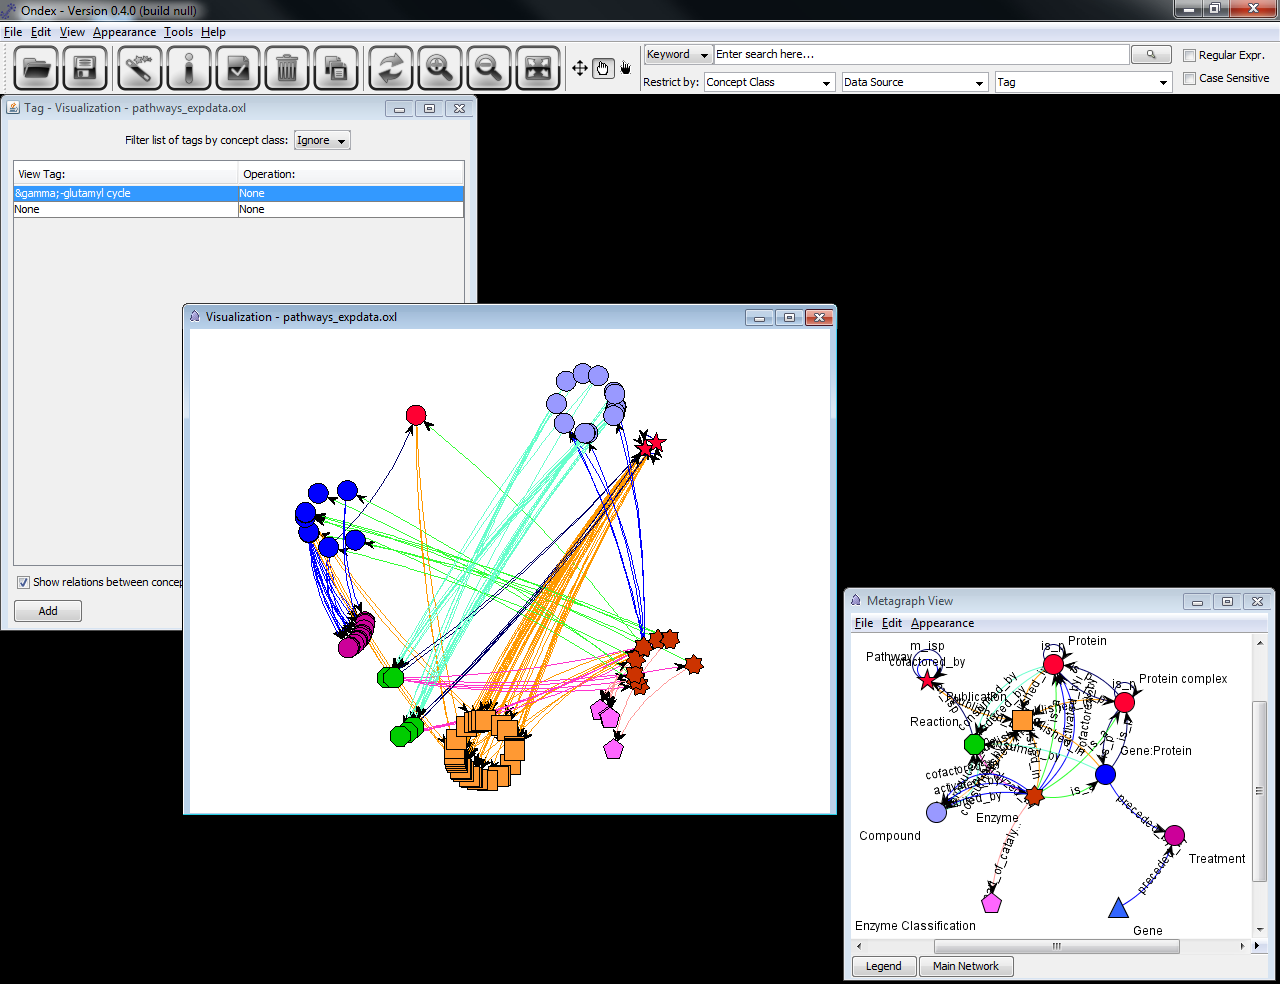
\includegraphics[scale=0.35]{images/Oct12/app1fig4.png} 
\caption{Tag filter results}
\label{fig:tag_result}
\end{figure}

The Gem layout (Appearance $->$ Layouts $->$ Gem) can easily be applied to this smaller network, which produces a more pleasant representation of the network
(see Figure \ref{fig:tag_gem}).

\begin{figure}[H]
\centering
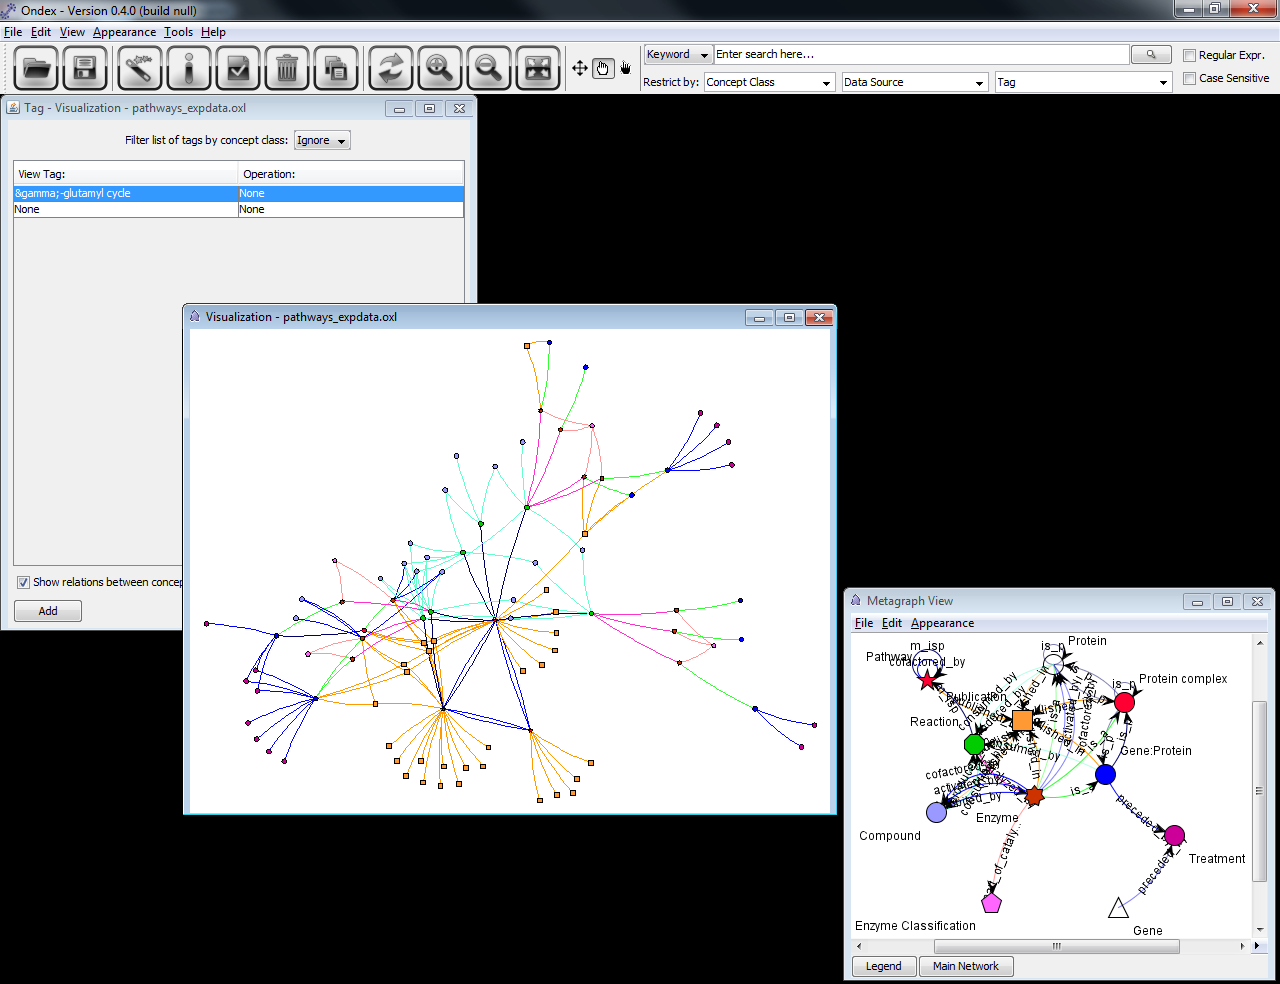
\includegraphics[scale=0.35]{images/Oct12/app1fig5.png} 
\caption{After applying the Gem layout}
\label{fig:tag_gem}
\end{figure}

Now additional features like displaying concept and relation labels (Appearance $->$ Labels) 
and anti-aliased painting (Appearance $->$ Smooth Relations) can be turned on to enrich the current visualisation. 
Using the Mouse wheel you can zoom into the network view. Try to locate a group of ``membrane alanyl aminopeptidases'' (see Figure \ref{fig:membrane}).

\begin{figure}[H]
\centering
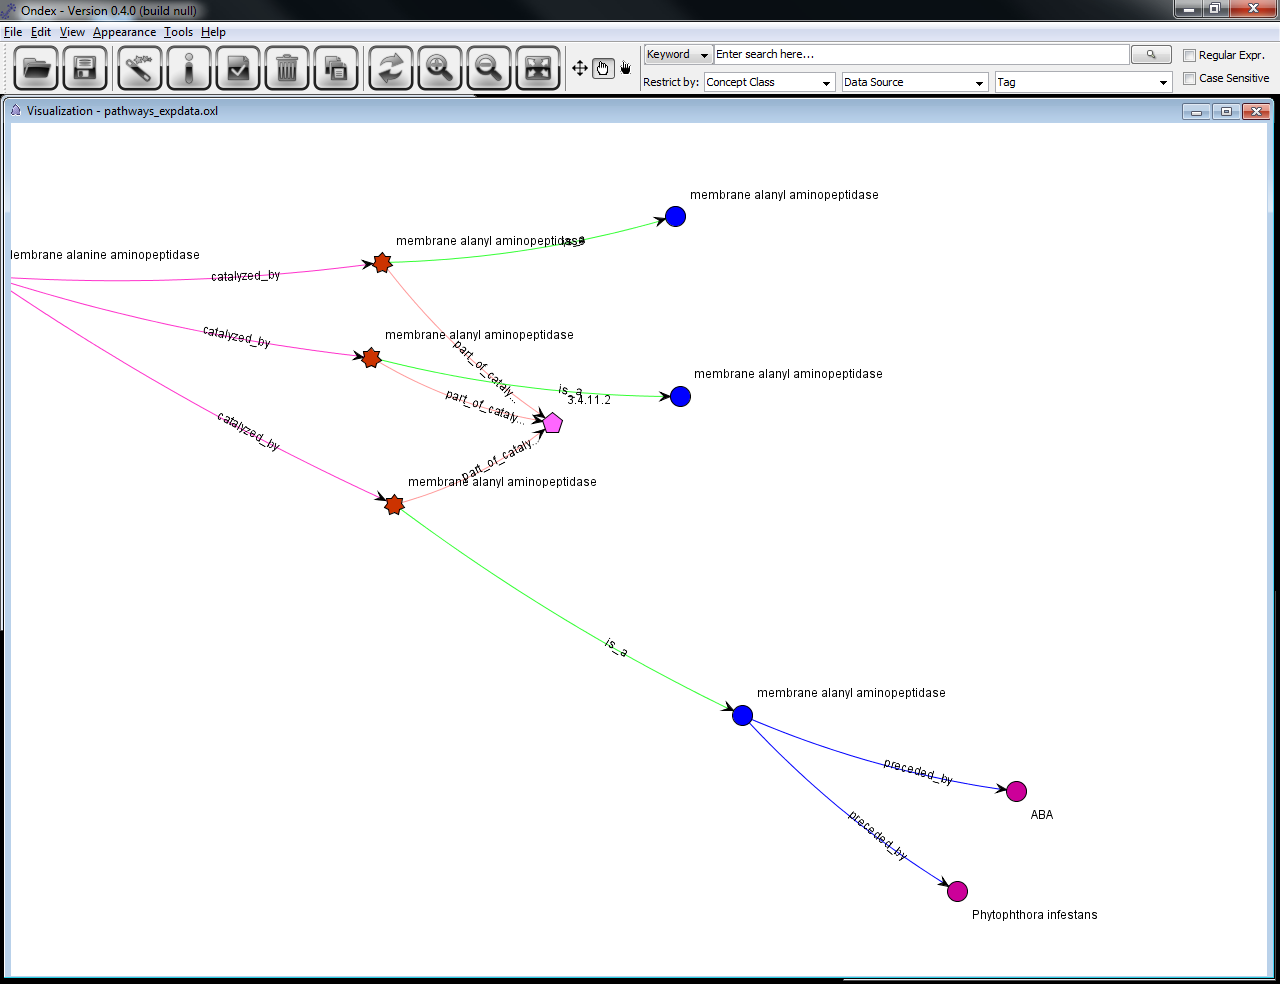
\includegraphics[scale=0.35]{images/Oct12/app1fig6.png} 
\caption{After zooming in}
\label{fig:membrane}
\end{figure}

Here only one Gene (blue circle) has information associated from the DRASTIC databases (purple circle). 
On all of these three genes additional information can be displayed by right-clicking on a concept (see Figure \ref{fig:properties}).

\begin{figure}[H]
\centering
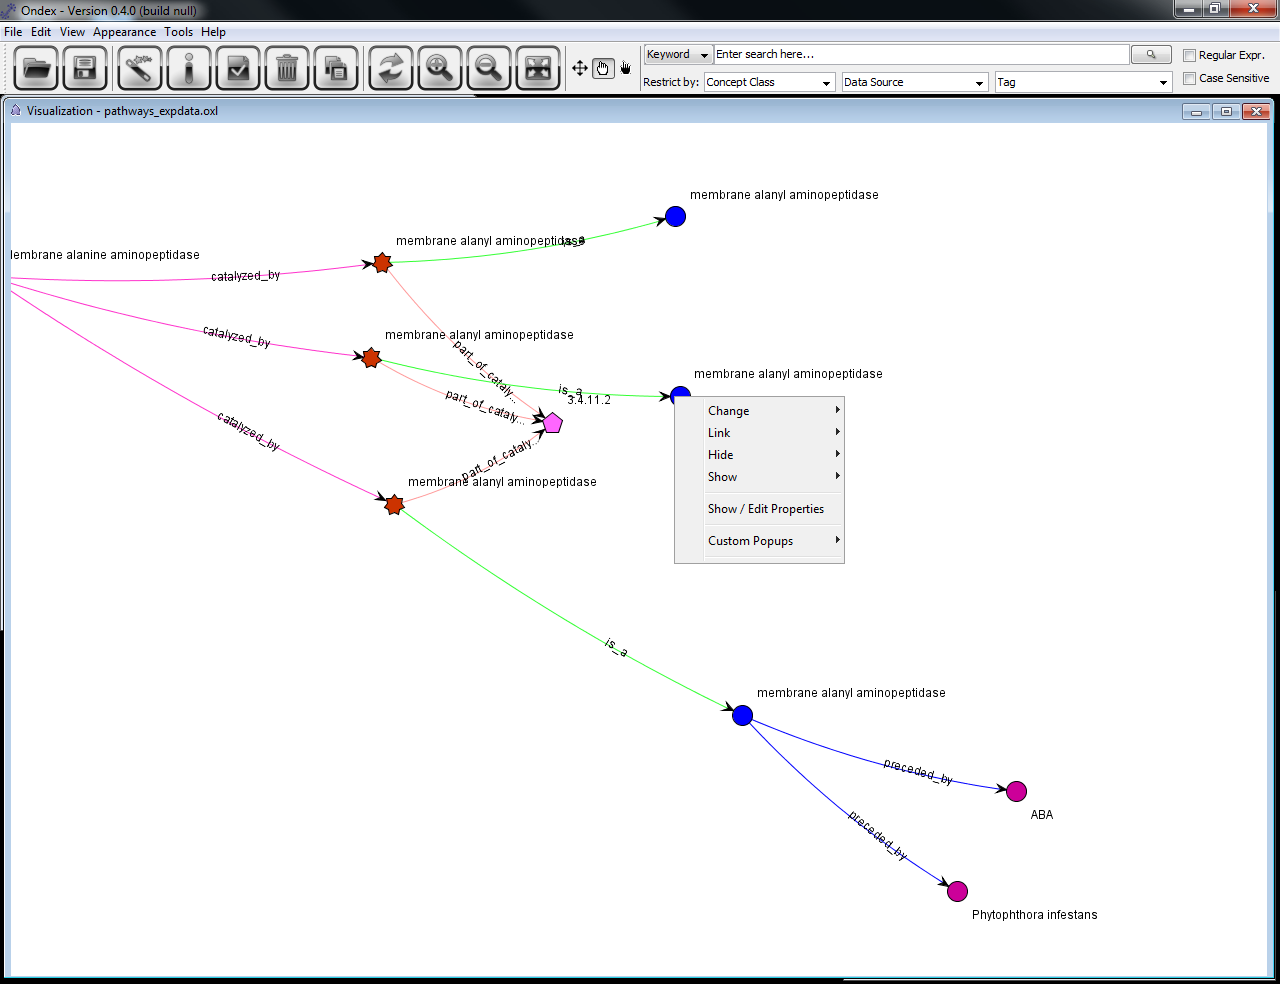
\includegraphics[scale=0.35]{images/Oct12/app1fig7.png} 
\caption{Concept properties}
\label{fig:properties}
\end{figure}

By clicking on ``Show / Edit Properties'' you are able to inspect all the properties assigned to this concept. 
Selecting ``View/Edit Concept Attributes'' displays a tab based representation of all values of the attributes (see Figure \ref{fig:gds}).

\begin{figure}[H]
\centering
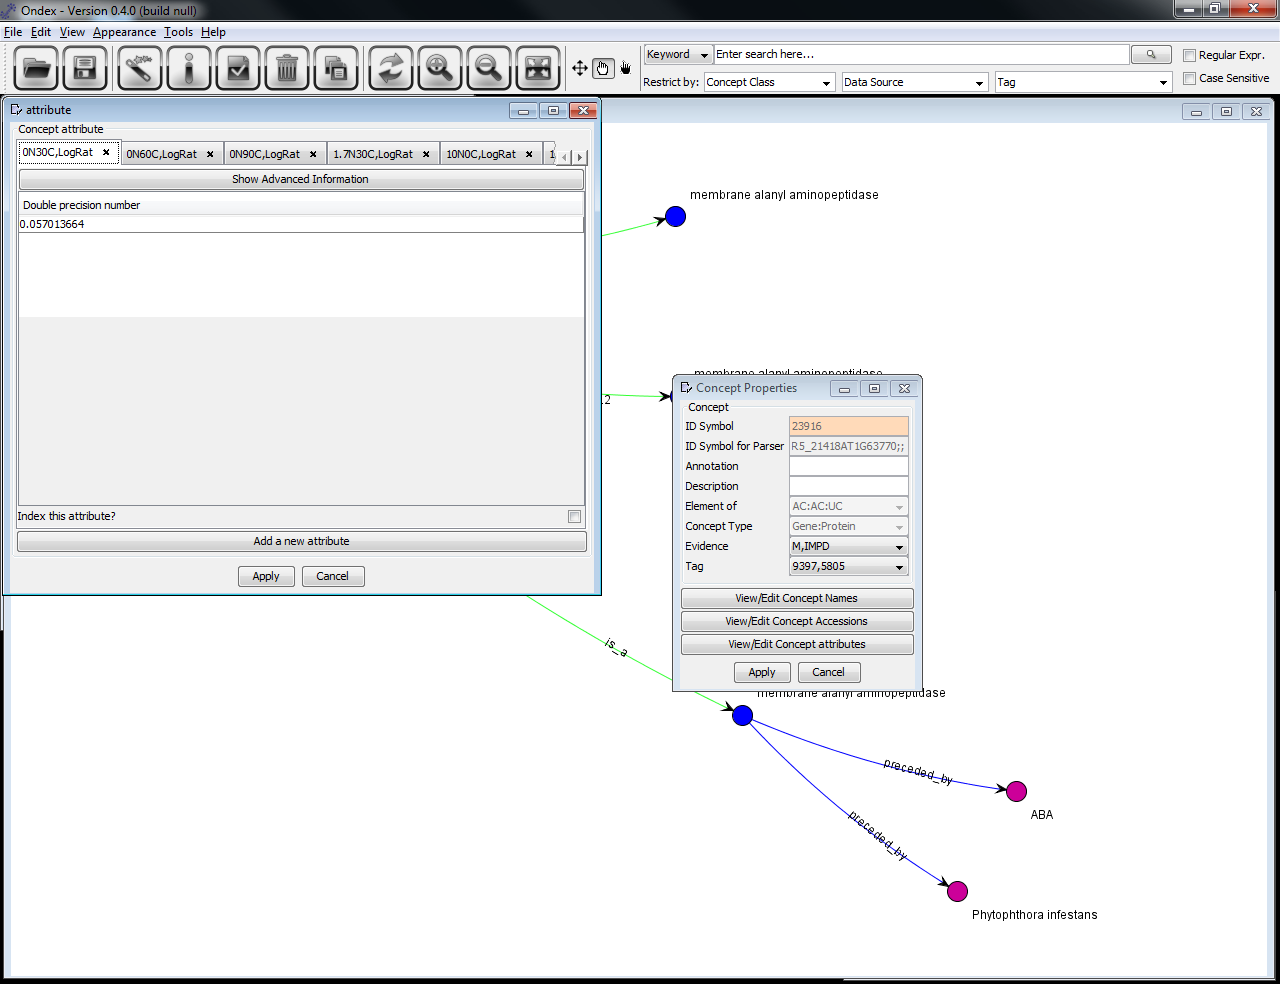
\includegraphics[scale=0.35]{images/Oct12/app1fig8.png} 
\caption{Concept attributes}
\label{fig:gds}
\end{figure}

In this case the values of the attributes are the microarray expression data listed according to the treatment. 
Now we can use the ``Scale Concepts by Numerical Value'' annotator (Tools $->$ Annotators $->$ Scale Concepts by Numerical Value) 
to actually map the values of the attributes to the visualisation of the corresponding concepts (see Figure \ref{fig:scale}).

\begin{figure}[H]
\centering
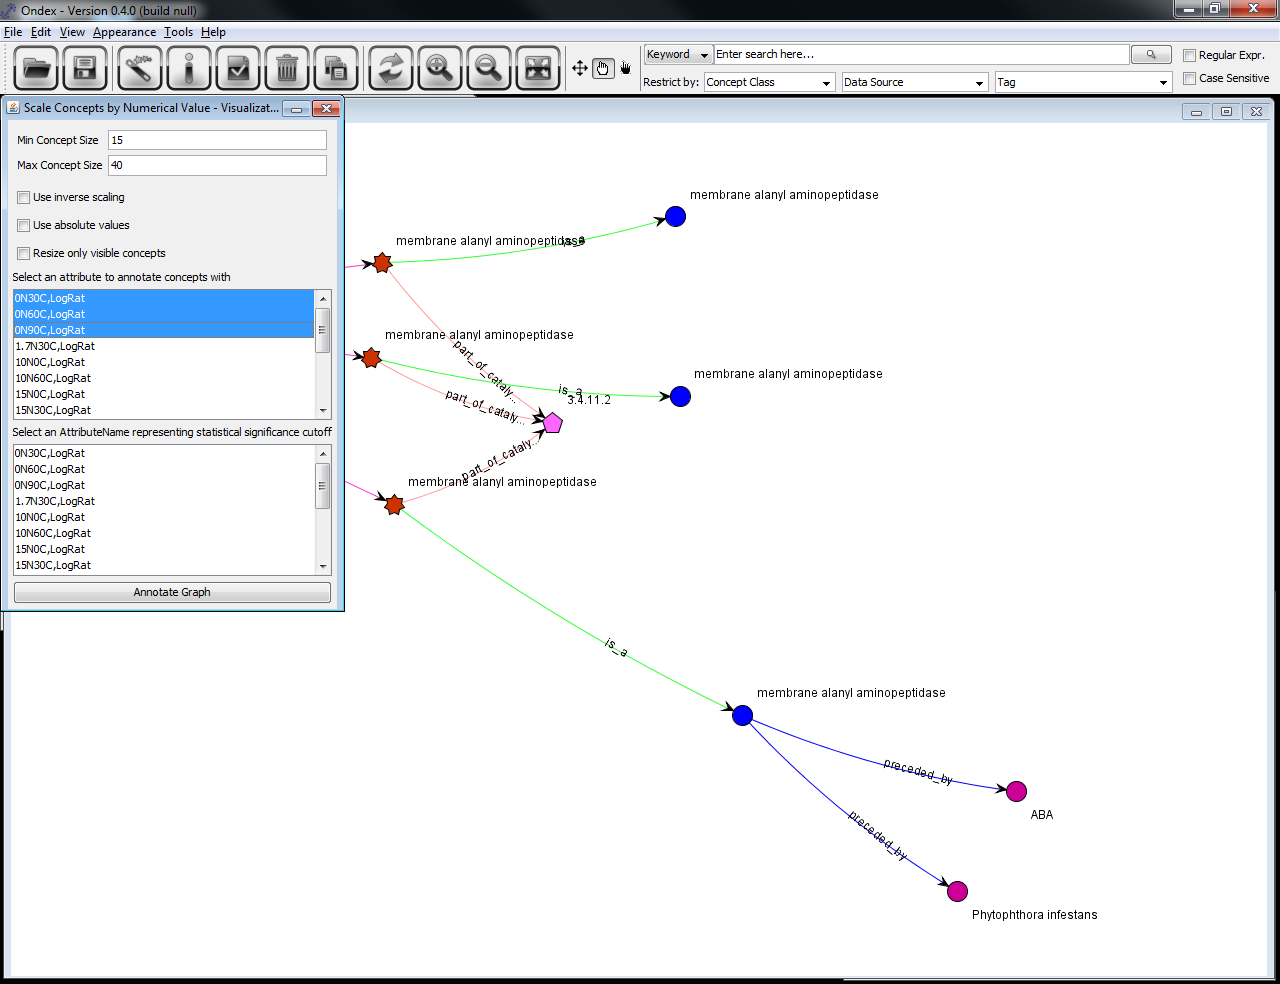
\includegraphics[scale=0.35]{images/Oct12/app1fig9.png} 
\caption{Scale Concept by Numerical Value annotator}
\label{fig:scale}
\end{figure}

The annotator supports multiple value selection. 
Here all treatments of the form 0NxC are selected. 
Annotate Graph performs the changes to the visualisation.
Figure \ref{fig:scale_results} shows the results.

\begin{figure}[H]
\centering
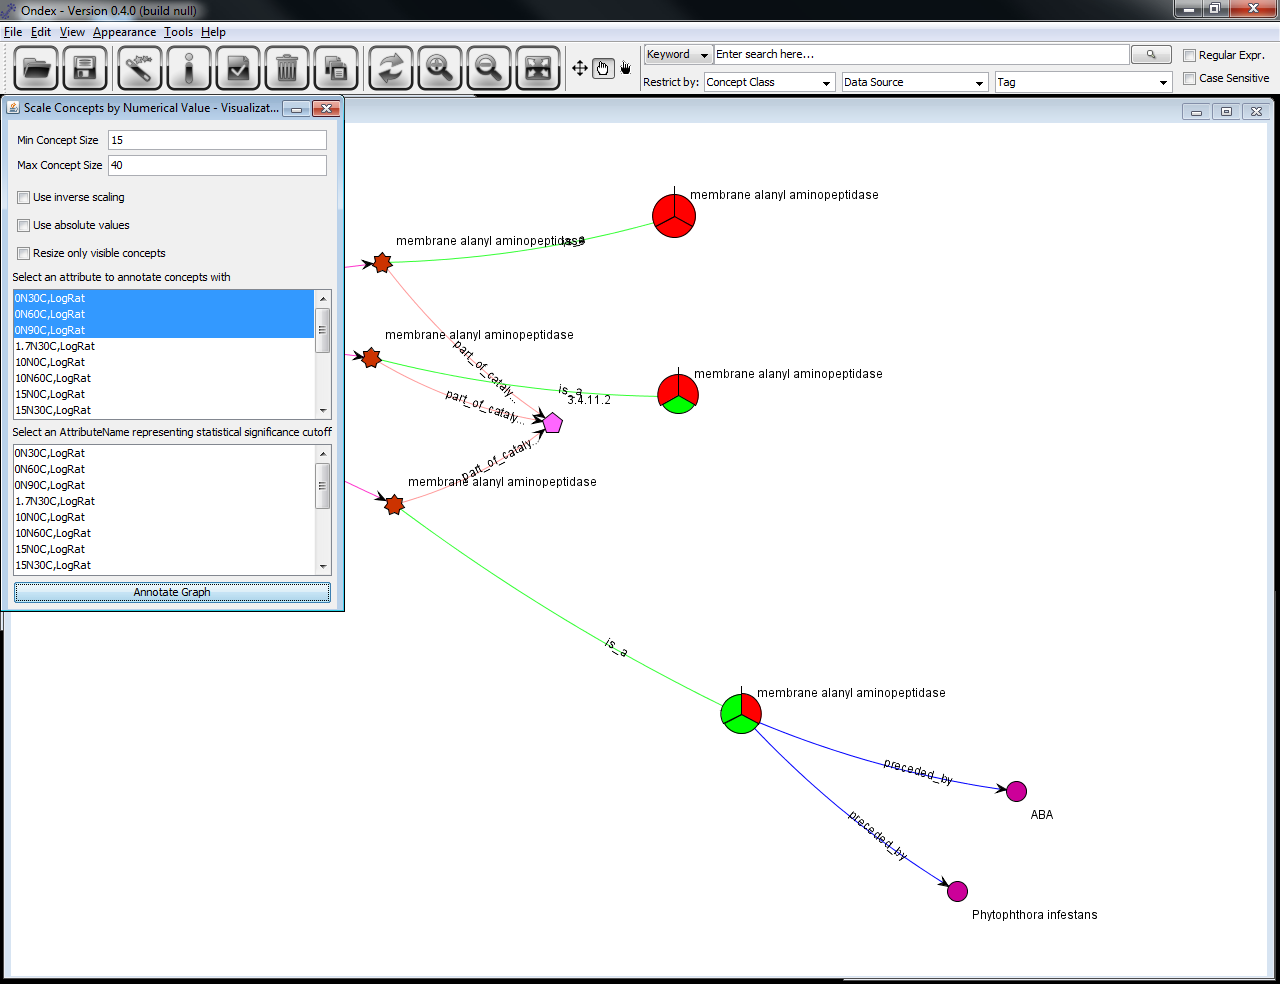
\includegraphics[scale=0.35]{images/Oct12/app1fig10.png} 
\caption{Results of the Scale Concept by Numerical Value annotator}
\label{fig:scale_results}
\end{figure}

The visualisation for the concepts now changed to pie charts. 
The pie chart is divided into the number of treatments that were selected in the annotator. 
It displays information from the top clockwise in the order in which they appear in the annotator
(it is possible to drap and drop the order around in the annotator). 
Visual inspection of this network now reveals that the gene at the top shows a constant expression pattern, 
whereas the other two Genes are differently regulated (red for up-regulation and green for down-regulation).

\begin{figure}[H]
\centering
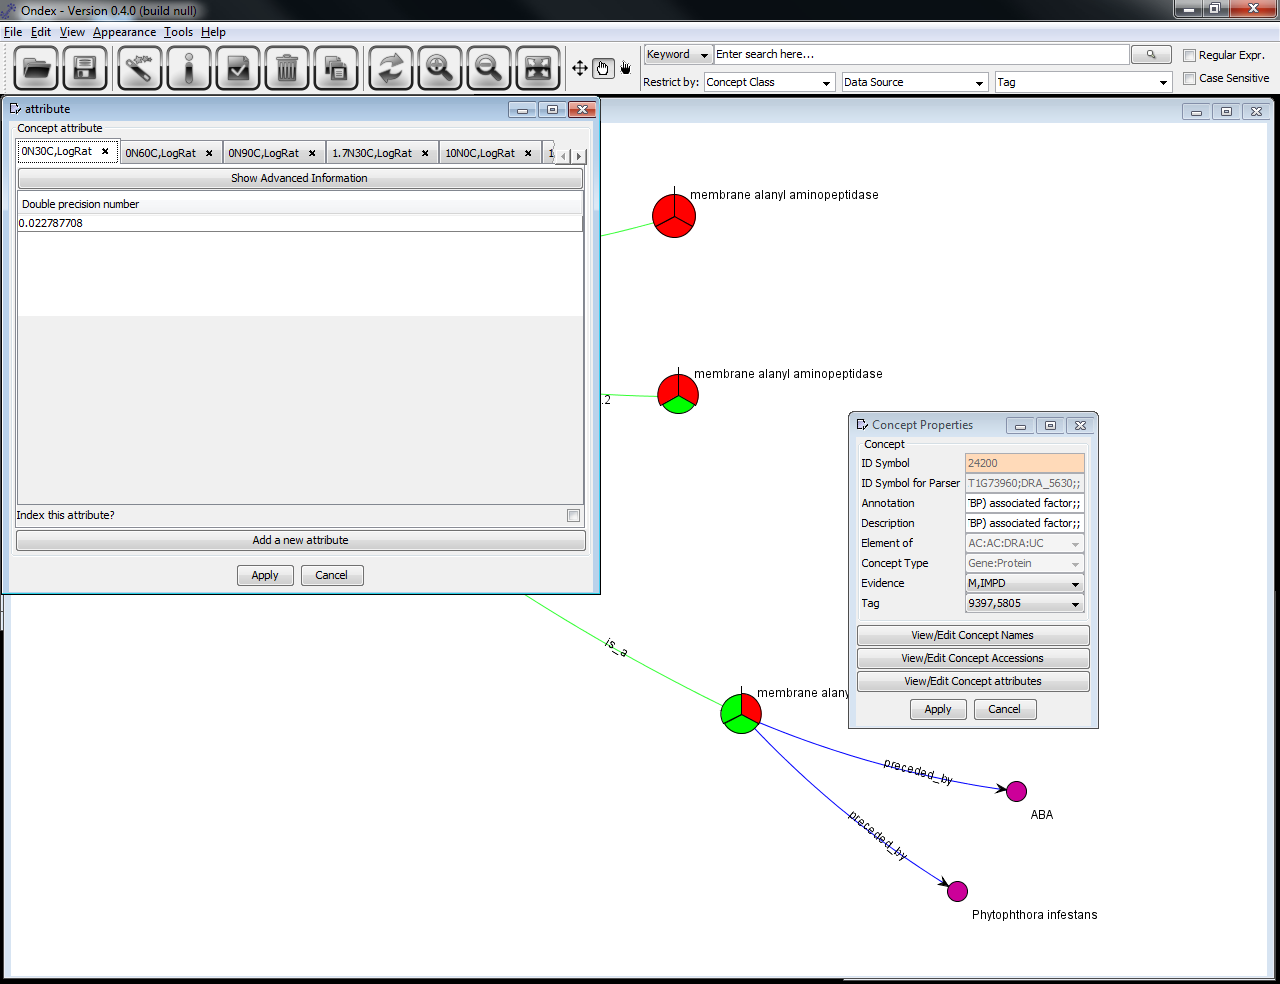
\includegraphics[scale=0.35]{images/Oct12/app1fig11.png} 
\caption{Further analysis}
\label{fig:further}
\end{figure}

Further inspection (see Figure \ref{fig:further}) of the attribute's value of the bottom gene supports the hypothesis 
that the up measurement might be wrong and the Gene might have been down-regulated across all three conditions. 
In addition we can annotate this gene with information from the DRASTIC database showing that 
this particular gene has a significant change in expression under the associated conditions. 

It is also possible to have a second visualisation window showing the same graph with different annotations.
To do so, use the 7th icon (``Copy whole Network as new'') or use the Edit menu -$>$ Clone Network.
A question will pop up ``Do you want to link views?''. 
If you answer no, the whole graph will load up using the circular layout.
If you answer yes, the concepts/relations visible in your current visualisation window will appear in the second one (at the same positions),
as shown in Figure \ref{fig:copygraph}.

\begin{figure}[H]
\centering
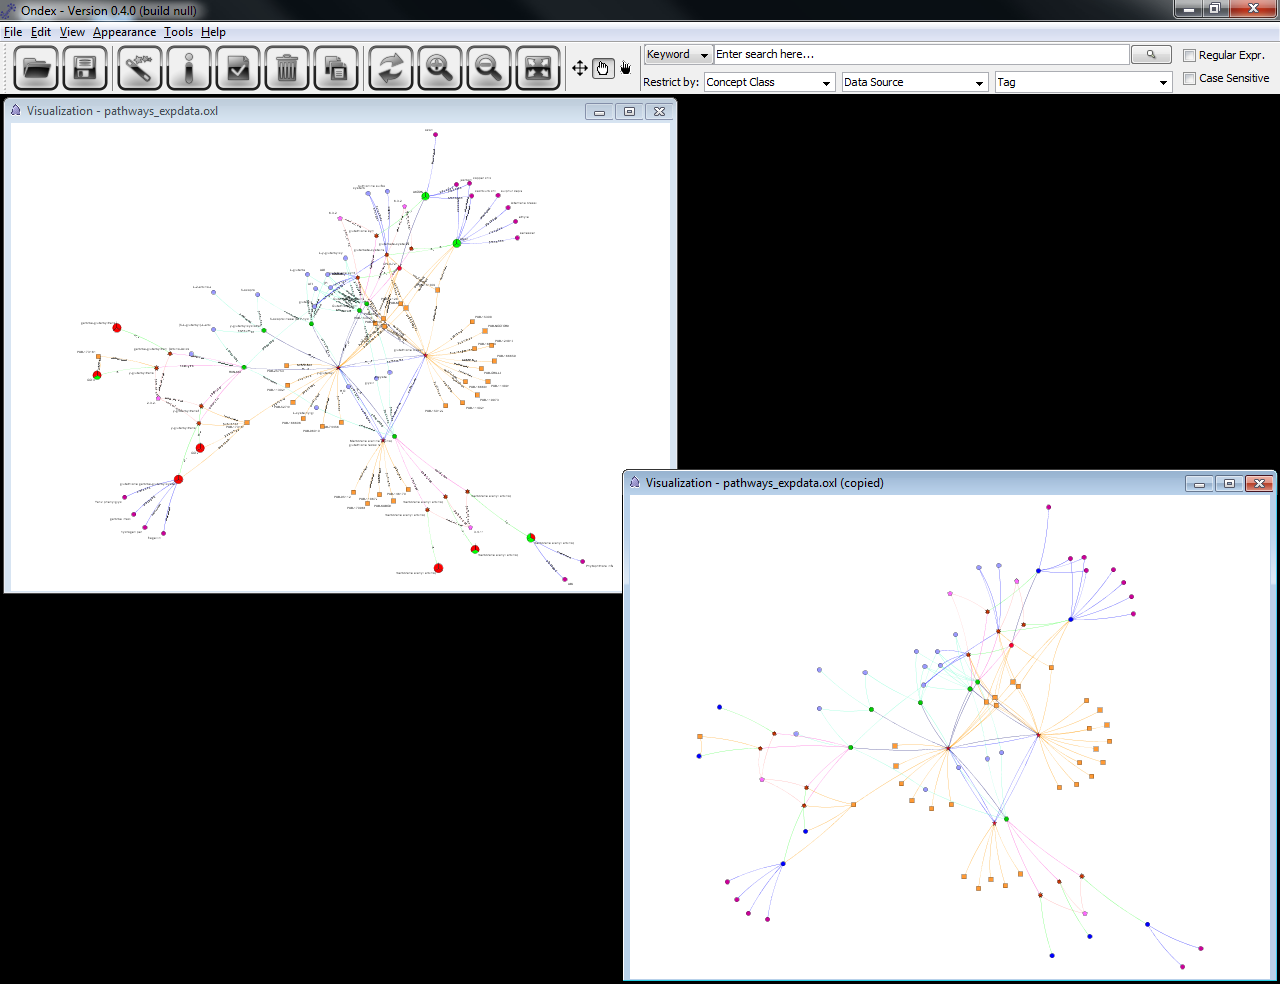
\includegraphics[scale=0.35]{images/Oct12/app1fig12.png} 
\caption{Copy whole graph}
\label{fig:copygraph}
\end{figure}

Figure \ref{fig:clone} shows how moving concepts happen in both windows from then on
and that different annotations can be displayed.

\begin{figure}[H]
\centering
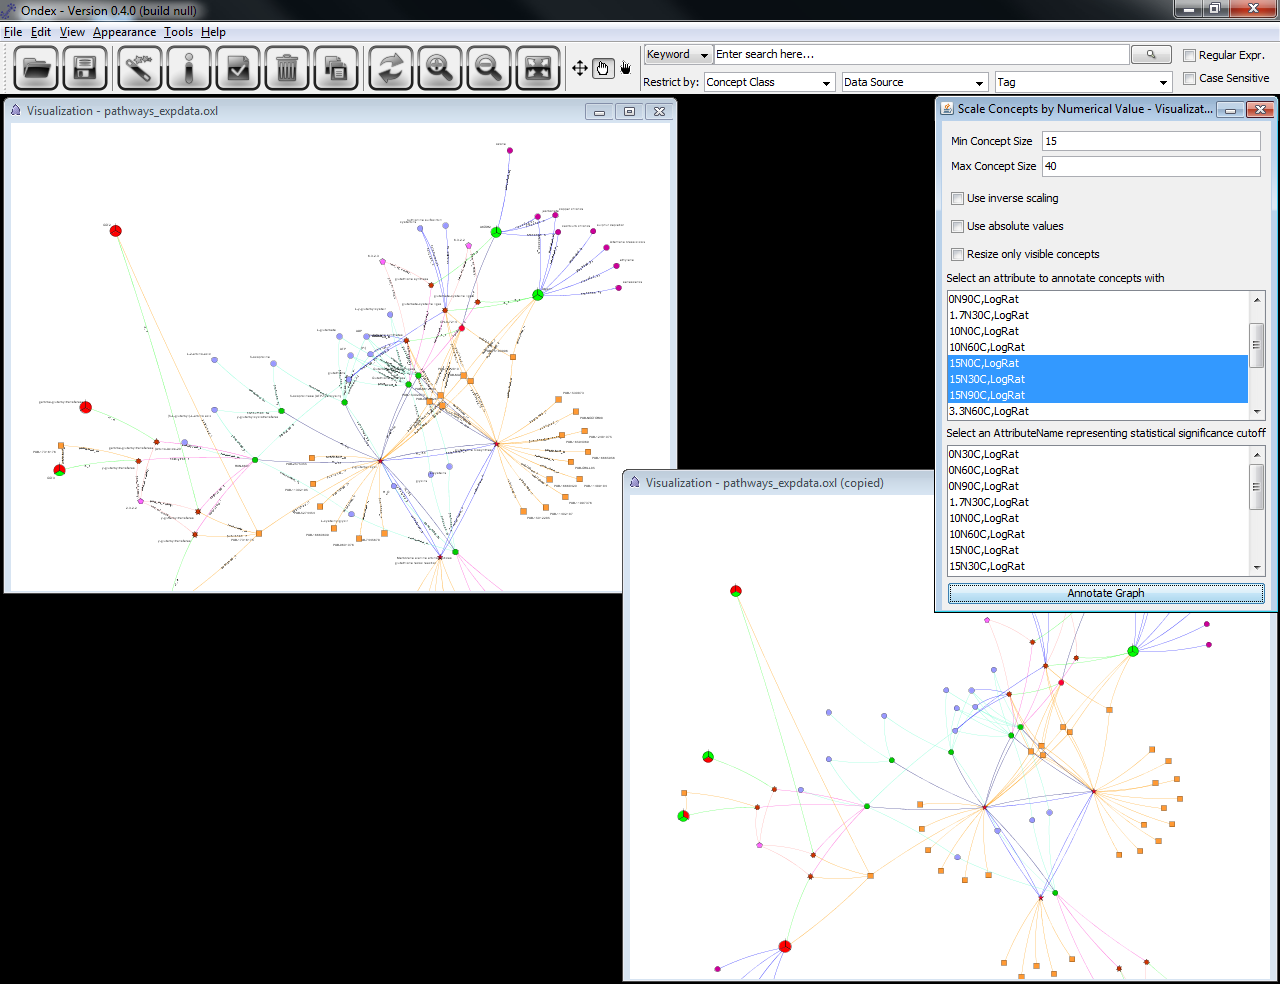
\includegraphics[scale=0.35]{images/Oct12/app1fig13.png} 
\caption{Layout is linked across both windows}
\label{fig:clone}
\end{figure}

{\em{Summary}}\\
In this example, we showed how visualisation of expression patterns can leverage the understanding 
in terms of comparing conditions and influence on pathways. We identified one particular Gene with an irregular expression pattern. 
Furthermore, data integration helped to enrich pathways from AraCyc with information about influential treatments from DRASTIC. 